\chapter{BENCHMARK OF EFFECTIVENESS OF IMAGE ATTACK METHODS AGAINST DEFENDED POLICIES}
\label{sec:exp3}

This section reports the results of the last of the three experiments included in this thesis. It benchmarks the effectiveness of different image attacks used by two different policy attacks to decrease victim's rewards. The victim models have been protected with different defense mechanisms. 

\section{Benchmark of the effectiveness of image attack methods against defended policies}
The last experiment included in this work consists of a benchmark to evaluate the robustness of defended policies trained with DQN on the environment of Pong. All policies have been attacked with the white-box image attack FGSM under a fixed threat model. This work compares the {\it reward vs perturbation} and {\it accuracy vs perturbation} curves of the defended victim policies by attacking them over increasing values of perturbations’ strength. Policies have been defended with the following defense methods:
\begin{itemize}
    \item FGSM adversarial training;
    \item PGD adversarial training;
    \item JPEG conversion;
    \item Feature squeezing (Bit squeezing);
    \item No defense.
\end{itemize}
Note that in the benchmark is also included an undefended version of the victim policy so as to have a comparison of the defended policies with the undefended one. 
Policies have been attacked with three different white-box image attacks methods including:
\begin{itemize}
    \item FGSM;
    \item PGD;
    \item MI (Momentum Iterative);
    \item No attack.
\end{itemize}
The {\it no attack} method which corresponds to evaluating the target policy without attacking it at all has been introduced so to compare the effect of each attack method with respect to not attacking at all. The curves have been generated attacking with both untargeted and targeted attacks and their corresponding results are reported in two different sections.

\subsection{Experiments settings}
\subsubsection{Defenses hyper-parameters}
Two of the four defenses that have been included in the benchmark consist of adversarial training with FGSM and PGD respectively. The first policy is the same policy trained with DQN used in the experiment in section \ref{sec:exp2}. The policy protected with PGD adversarial training has been trained crafting adversarial perturbations with 10 iterations of PGD. Besides the type of attack and the number of iterations, there is no difference between the way adversarial training has been applied. Perturbations have been crafted under \(l_\infty\) norm and \(\epsilon\) fixed to 0.01. 

The third defense that has been implemented is a simple method that converts each observation to JPEG format before feeding it to the network. JPEG images retain 20\% of the quality of the original observations. 

The fourth method is known as feature squeezing and it consists of reducing the number of features of each pixel for each observed image. Since we are dealing with gray-scale images, what we are going to reduce is the number of bits to represent each pixel, thus we may sometimes refer to this method as bit squeezing. More specifically, it reduces the number of bits from 8 to 5, thus lowering the number of features from \(2^8\) to \(2^5\). This method shrinks the number of features by 80\% with respect to the original observations.

In this benchmark we have evaluated a powerful defense method such as adversarial training and two simple defenses such as JPEG conversion and feature squeezing so to test defenses with different levels of effectiveness.

\subsubsection{Image adversarial attacks settings}
This section reports the value of the hyper-parameters adopted in the image attacks included in the benchmark. Note that this time the perturbation strength \(epsilon\) is variable. The first attack, FGSM, has already been employed in the previous experiments and its hyper-parameters are maintained the same for this work. The two iterative methods PGD and MI execute 10 iterations each attack and each iteration refines the adversarial perturbations with \(epsilon_i\) (attack step size) of \(\epsilon/5\). 

The main reason why we have chosen the above-mentioned attacks is that they all work under targeted and untargeted settings and they support the three most common distance norms, namely \(l_\infty, l_1, l_2\). They also explicitly define the hyper-parameter \(\epsilon\) to limit the size of the adversarial perturbations. For example, adversarial examples crafted with C\&W method are not easily comparable in this benchmark since the method doesn't have a hyper-parameter \(\epsilon\) that can be fine-tuned. Moreover, those attacks are well-studied and commonly used in research papers, thus proving to work well in practice and worth being evaluated.

\subsubsection{Threat model}
All methods included in this benchmark are evaluated under both untargeted and targeted settings. Adversarial examples are crafted using the \(l_\infty\) distance norm. Their perturbations' strength \(\epsilon\) ranges from 0 to 0.05 included with a step size of 0.005. Curves are generated by computing the rewards of the policy under attack and the success rate of the malicious attacks according to the value of \(\epsilon\) defined in correspondence of each point.

\subsection{Benchmark of untargeted white-box attacks}
The charts relative to the {\it reward vs perturbation} and {\it accuracy vs perturbation} curves obtained under untargeted settings are shown in figures \ref{figure:untargeted-rew} and \ref{figure:untargeted-suc} respectively. When attacking the policy protected with FGSM adversarial training, MI is the attack that results most effective followed by PGD and FGSM. It is interesting to note that although adversarial training has been conducted with \(\epsilon\)=0.01, adversarial training can still protect quite well against adversarial observations crafted with higher values of perturbation strength. The defense is completely broken for noise generated with \(\epsilon\) greater than 0.03. Conversely, when attacking PGD adversarial training, FGSM and PGD perform the best but the difference between the three attack methods is never too significant. PGD struggles to reduce the reward of the agent against JPEG filter and bit squeezing with respect to the other two attack methods which perform very similar. FGSM is also the only attack that can't reduce the average reward to \(-20\) when attacking the undefended policy. When comparing the success rate of the three methods, PGD is the attack the overall performs the best and FGSM is the worst. In particular, PGD adversarial training seems to be more robust against FGSM, and bit squeezing is more vulnerable against PGD attack. When attacking FGSM adversarial training and JPEG filer, all the attacks show a similar success rate.

It is interesting to note that when attacking JPEG filter and bit squeezing, all attacks seem to break the defense right after increasing the strength of the perturbations to be greater than 0.01. In fact, after this threshold, their curves drop to -20 points and the attack accuracy skyrockets to be 100\%. The two defenses based on adversarial training are better at improving the robustness of their policies. As we can see from the charts, the average rewards still begin decreasing when \(\epsilon\) is greater than 0.02 or 0.03 but both curves approach -20 with a more gentle descent. Conversely, the attack accuracy against the same defenses steadily increases over the whole perturbations range but the rise is never too steep.


\begin{figure}
  \centering
  \subcaptionbox{FGSM adversarial training\label{fig:subfig-a}}
    {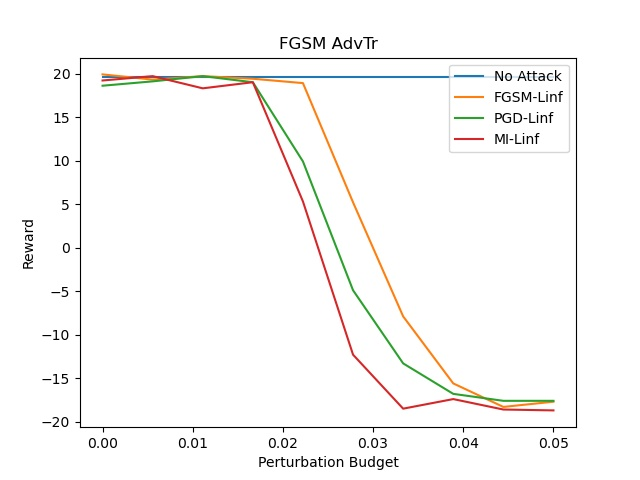
\includegraphics[width=0.49\linewidth]{images/exp3/untargeted/FGSM_AdvTr.jpg}}
  \subcaptionbox{PGD adversarial training\label{fig:subfig-b}}
    {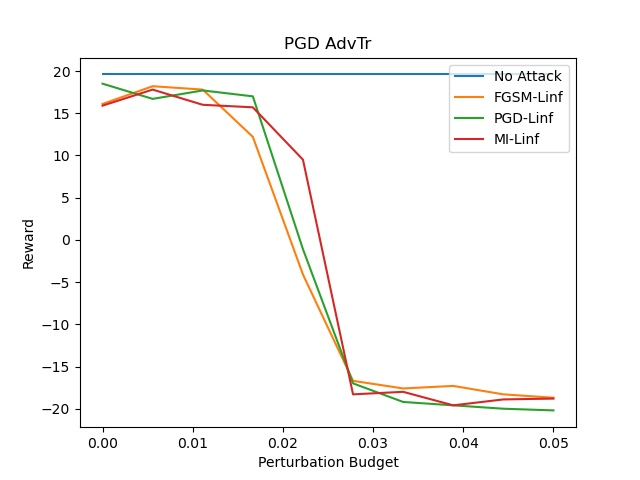
\includegraphics[width=0.49\linewidth]{images/exp3/untargeted/PGD_AdvTr.jpg}}
  \subcaptionbox{JPEG filter\label{fig:subfig-c}}
    {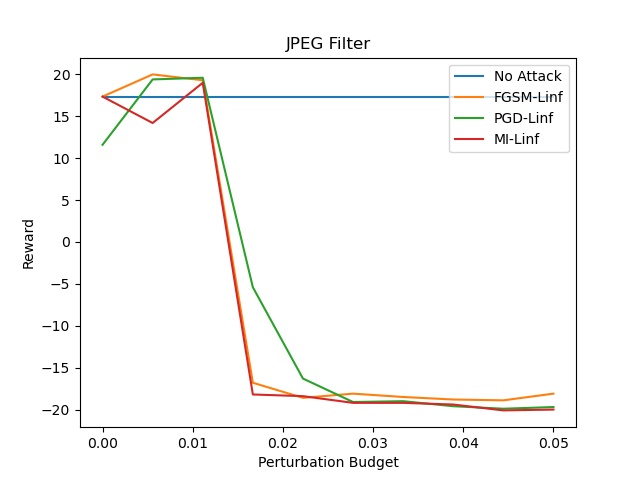
\includegraphics[width=0.49\linewidth]{images/exp3/untargeted/JPEG_Filter.jpg}}
  \subcaptionbox{Bit squeezing\label{fig:subfig-d}}
    {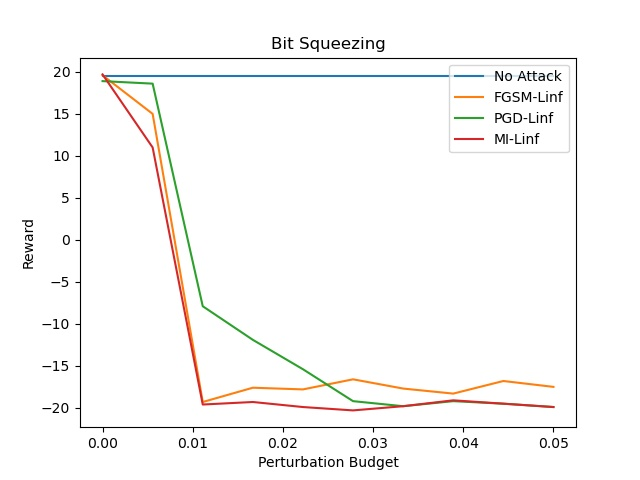
\includegraphics[width=0.49\linewidth]{images/exp3/untargeted/Bit_Squeezing.jpg}}
  \subcaptionbox{No Defense\label{fig:subfig-e}}
    {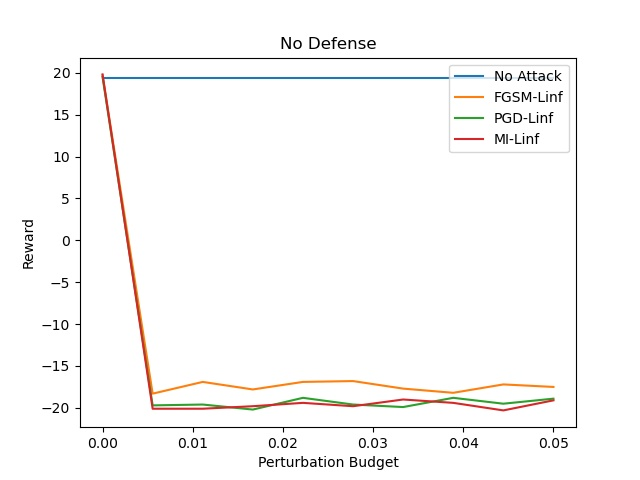
\includegraphics[width=0.49\linewidth]{images/exp3/untargeted/No_Defense.jpg}}
  \caption{The {\it reward vs perturbation} curves of 5 DQN policies trained to play Pong and defended with 5 different defense methods (including no defense) under the \(l_\infty\) norm attacking with increased perturbations strength. Perturbations have been crafted in an untargeted way.}
  \label{figure:untargeted-rew}
\end{figure}

\begin{figure}
  \centering
  \subcaptionbox{FGSM adversarial training\label{fig:subfig-a}}
    {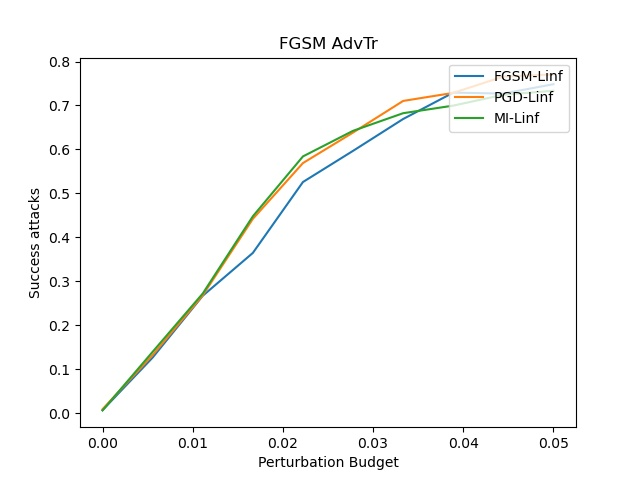
\includegraphics[width=0.49\linewidth]{images/exp3/untargeted/FGSM_AdvTr_succ.jpg}}
  \subcaptionbox{PPO adversarial training\label{fig:subfig-b}}
    {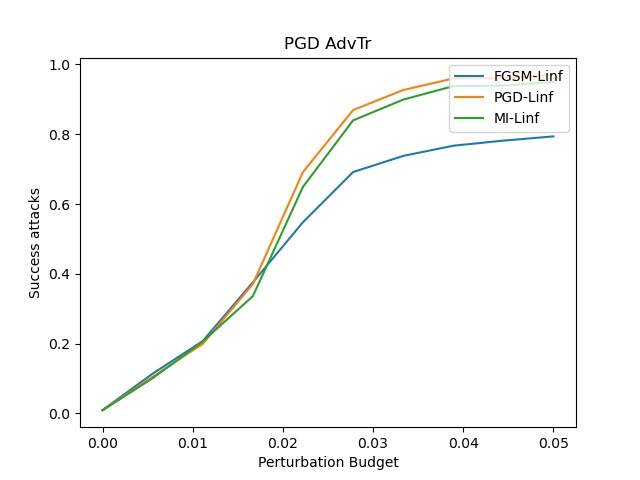
\includegraphics[width=0.49\linewidth]{images/exp3/untargeted/PGD_AdvTr_succ.jpg}}
  \subcaptionbox{JPEG filter\label{fig:subfig-c}}
    {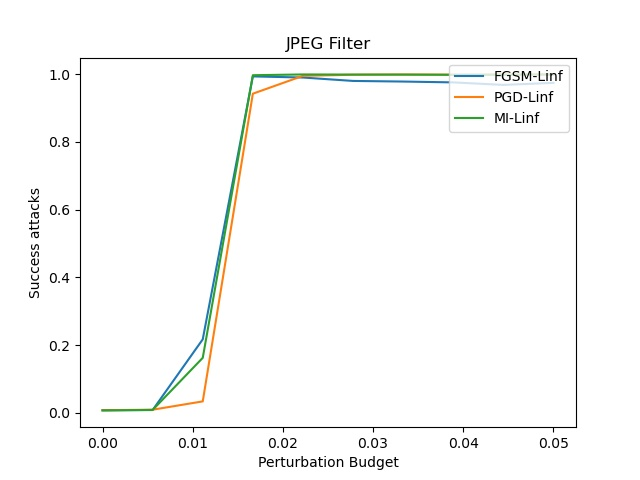
\includegraphics[width=0.49\linewidth]{images/exp3/untargeted/JPEG_Filter_succ.jpg}}
  \subcaptionbox{Bit squeezing\label{fig:subfig-d}}
    {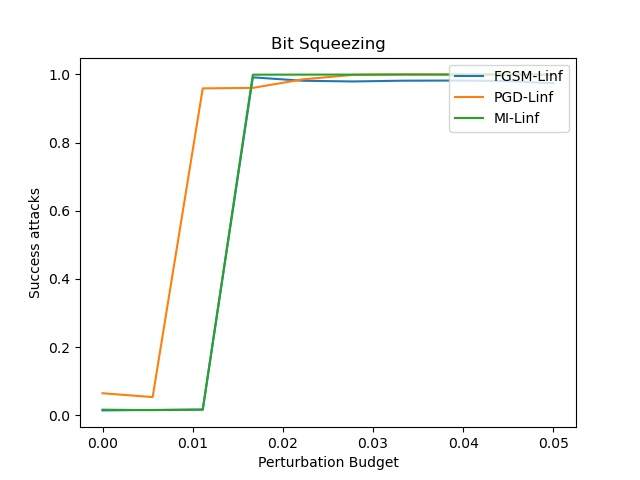
\includegraphics[width=0.49\linewidth]{images/exp3/untargeted/Bit_Squeezing_succ.jpg}}
  \subcaptionbox{No defense\label{fig:subfig-e}}
    {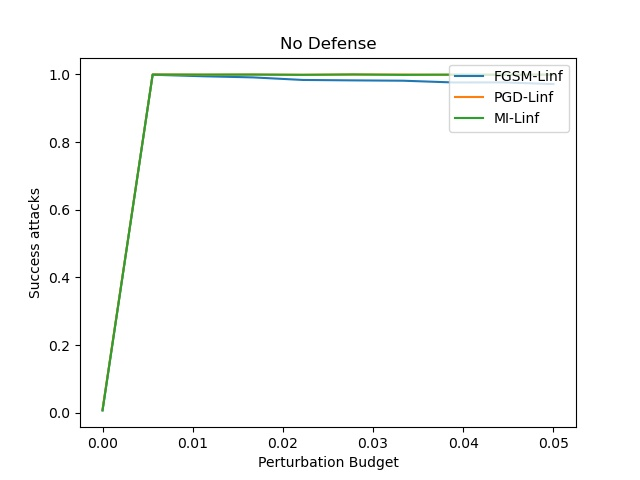
\includegraphics[width=0.49\linewidth]{images/exp3/untargeted/No_Defense_succ.jpg}}
  \caption{The {\it accuracy vs perturbation} curves of 5 DQN policies trained to play Pong and defended with 5 different defense methods (including no defense) under the \(l_\infty\) norm attacking with increased perturbations strength. Perturbations have been crafted in an untargeted way.}
  \label{figure:untargeted-suc}
\end{figure}

\subsection{Benchmark of targeted white-box attacks}
The charts relative to the {\it reward vs perturbation} and {\it accuracy vs perturbation} curves obtained under targeted settings are shown in figures \ref{figure:targeted-rew} and \ref{figure:targeted-suc} respectively. For each observation, the targeted action that has been selected is the action with the lowest probability. Hence, it is equal to adopt strategically-timed attack attacking all the possible observations. In terms of reward, FGSM is the attack that performs the worst against the two adversarial training-based defenses while the other two attacks obtain similar results. As for JPEG filter defense, the chart doesn't present any substantial difference among the curves of the evaluated attack methods. PGD is also the best attack to break bit squeezing defense. All curves begin to drop down for perturbations greater than 0.01 and the descent is steeper for JPEG filter and bit squeezing. As it was for the untargeted case, the value of the curves of the adversarial training-based defenses decreases more gradually and eventually reaches the bottom when \(\epsilon\) gets close to 0.03 or 0.04. The difference in terms of performance between adversarial training and the other two defenses is more significant when comparing their success rate curves. In fact, in the perturbations' strength interval taken into examination, targeted attacks against adversarial training protected policies work at most 20\% of the times while attacks against the other two defenses have a success rate of 100\% for \(\epsilon\) greater than 0.01. Under targeted settings, FGSM is the only attack whose accuracy never reaches 100\% against the undefended policy. It also shows an inferior performance against all the other defenses.

\begin{figure}
  \centering
  \subcaptionbox{FGSM adversarial training\label{fig:subfig-a}}
    {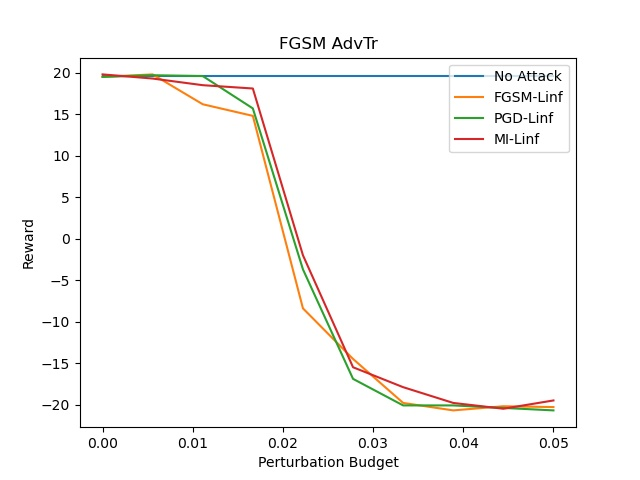
\includegraphics[width=0.49\linewidth]{images/exp3/targeted/FGSM_AdvTr.jpg}}
  \subcaptionbox{PPO adversarial training\label{fig:subfig-b}}
    {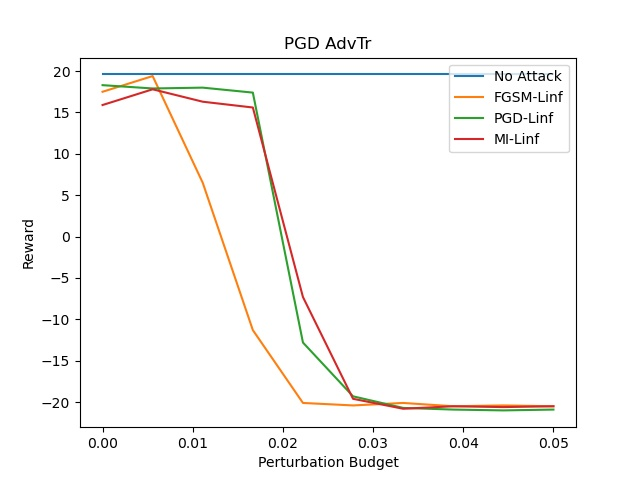
\includegraphics[width=0.49\linewidth]{images/exp3/targeted/PGD_AdvTr.jpg}}
  \subcaptionbox{JPEG filter\label{fig:subfig-c}}
    {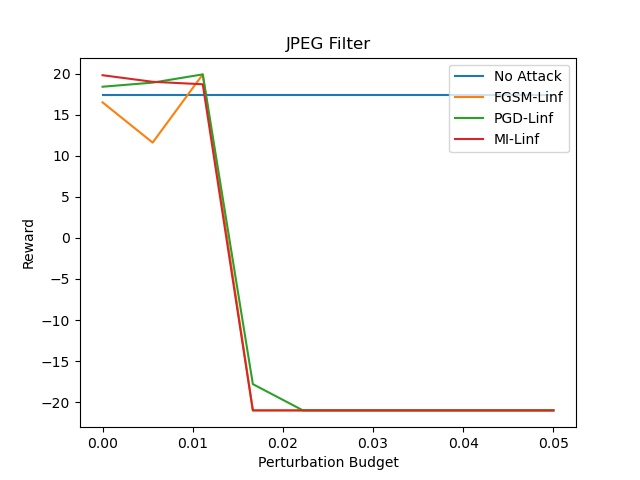
\includegraphics[width=0.49\linewidth]{images/exp3/targeted/JPEG_Filter.jpg}}
  \subcaptionbox{Bit squeezing\label{fig:subfig-d}}
    {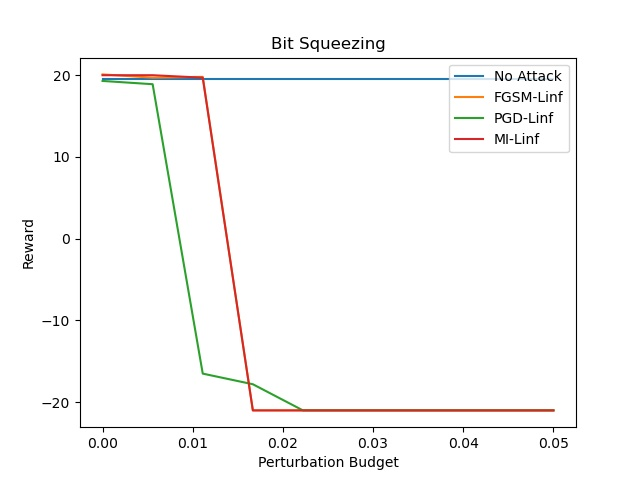
\includegraphics[width=0.49\linewidth]{images/exp3/targeted/Bit_Squeezing.jpg}}
  \subcaptionbox{No defense\label{fig:subfig-e}}
    {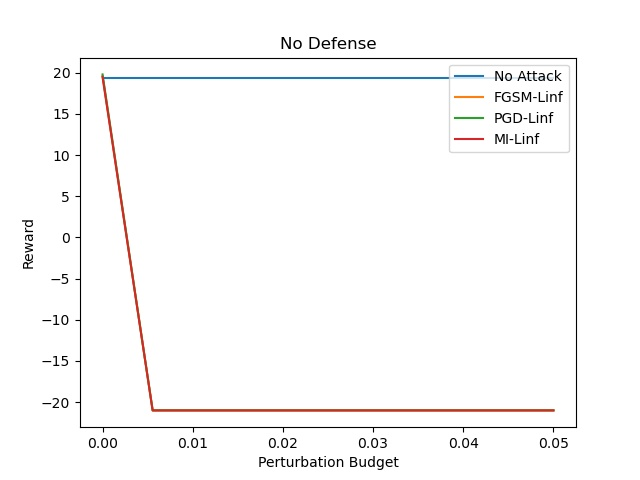
\includegraphics[width=0.49\linewidth]{images/exp3/targeted/No_Defense.jpg}}
  \caption{The {\it reward vs perturbation} curves of 5 DQN policies trained to play Pong and defended with 5 different defense methods (including no defense) under the \(l_\infty\) norm attacking with increased perturbations strength. Perturbations have been crafted in a targeted way.}
  \label{figure:targeted-rew}
\end{figure}

\begin{figure}
  \centering
  \subcaptionbox{FGSM adversarial training\label{fig:subfig-a}}
    {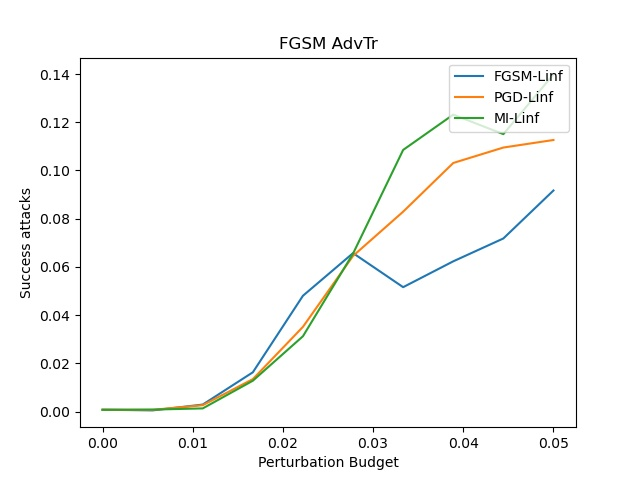
\includegraphics[width=0.49\linewidth]{images/exp3/targeted/FGSM_AdvTr_succ.jpg}}
  \subcaptionbox{PPO adversarial training\label{fig:subfig-b}}
    {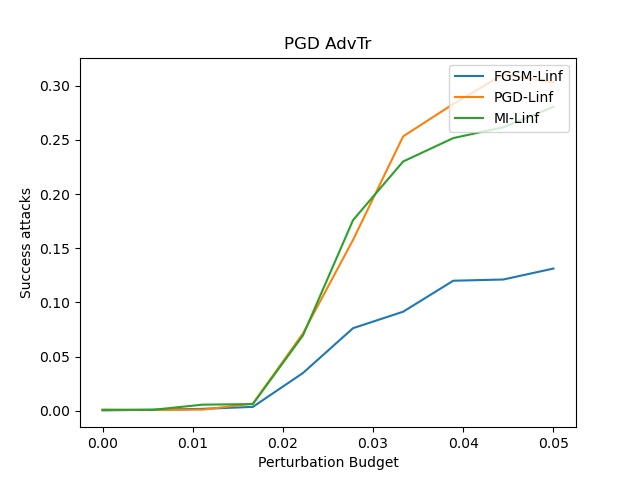
\includegraphics[width=0.49\linewidth]{images/exp3/targeted/PGD_AdvTr_succ.jpg}}
  \subcaptionbox{JPEG filter\label{fig:subfig-c}}
    {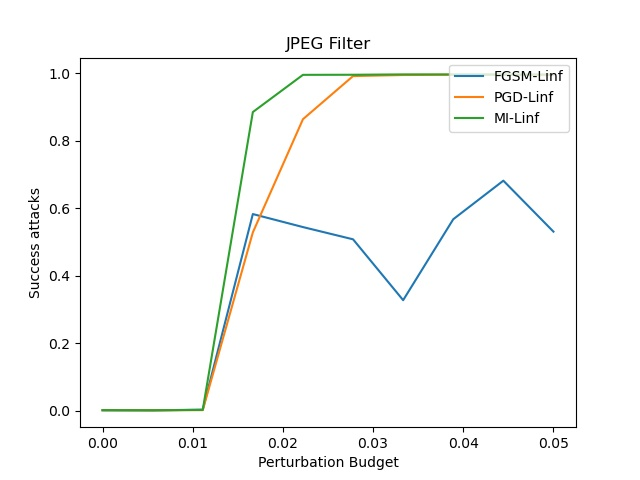
\includegraphics[width=0.49\linewidth]{images/exp3/targeted/JPEG_Filter_succ.jpg}}
  \subcaptionbox{Bit squeezing\label{fig:subfig-d}}
    {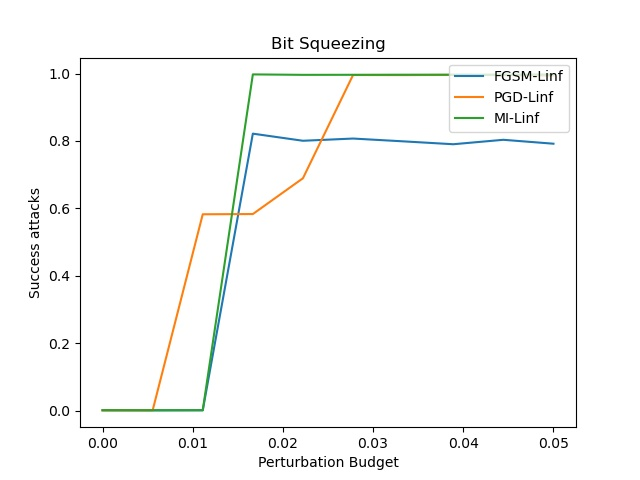
\includegraphics[width=0.49\linewidth]{images/exp3/targeted/Bit_Squeezing_succ.jpg}}
  \subcaptionbox{No defense\label{fig:subfig-e}}
    {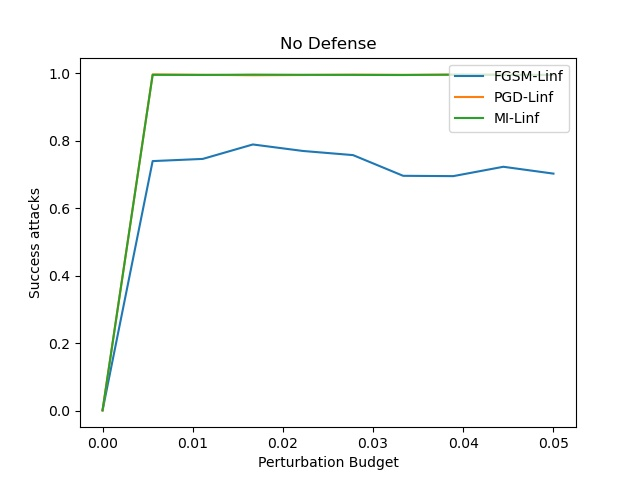
\includegraphics[width=0.49\linewidth]{images/exp3/targeted/No_Defense_succ.jpg}}
  \caption{The {\it accuracy vs perturbation} curves of 5 DQN policies trained to play Pong and defended with 5 different defense methods (including no defense) under the \(l_\infty\) norm attacking with increased perturbations strength. Perturbations have been crafted in a targeted way.}
  \label{figure:targeted-suc}
\end{figure}

\subsection{Findings}
This section shows the findings relative to the benchmark evaluated in this work. In particular, it makes some conclusions about the importance of this experiment, the differences between attacking under targeted and untargeted settings and it provides more insights about the evaluated defenses and their robustness.

\subsubsection{Importance of selecting the most appropriate image attack method}
Policy attacks based on image observations rely on image attacks to craft effective perturbations to fool their target agent. Hence, selecting the most effective image attack that performs better against a certain policy trained with a certain algorithm on a specific environment is a fundamental step to perform effective policy attacks.  In addition, different image attack methods might work better or worse against specific defense methods that protect the target policy. Thus, there are many variables that can condition the effectiveness of a policy attack. Also choosing the most appropriate threat model contributes to enhance the performance of the attacks and craft the most effective or imperceptible adversarial observations. For instance, in order to craft imperceptible adversarial examples, it is useful to know which minimal amount of \(\epsilon\) is enough to attack policy \(P\) defended with defense \(D\) on environment \(E\) or, given a fixed \(\epsilon\), it might be useful to find which attack shows the highest attack success rate or that reduces the agent's reward for the highest amount. Thus, reinforcement learning policies that take as input environment observations should have their robustness evaluated not only against policy attacks but also against image attack methods.

\subsubsection{Targeted and untargeted image attacks}
In this section, we are going to analyze the main differences that emerge when attacking under targeted and untargeted scenarios. Targeted attacks seem to be better at reducing the agent's reward but the probability that their attacks are executed correctly is significantly lower than their untargeted counterpart. However, they are still effective since most of the failed attacks, although they fail to fool the agent to select the selected action, they still corrupt the observations enough to fool the agent to take a random sub-optimal action. However, given a similar attack accuracy, targeted attacks can easily outperform untargeted attacks. For example, given the charts relative to the undefended policy, FGSM has 100\% accuracy under untargeted attack scenarios and a little more than 70\% accuracy under targeted settings. Nevertheless, its average reward for the untargeted case is a few points higher than its corresponding average reward obtained in the targeted scenario. This phenomenon is probably due to the fact that targeted attacks are more lethal and when they succeed they provoke greater damage to the victim policy. It is also worth noting that, in terms of accuracy, FGSM seems to suffer a loss in performance when attacking under targeted settings with respect to its targeted version. Overall, MI is the most effective attack under both settings. 

\subsubsection{Robustness of the evaluated defenses}
Among the evaluated policies, the most robust one seems to be the one defended with the two adversarial training-based methods, in fact, they offer great protection under both attack settings. PGD adversarial training is perhaps a little better than FGSM when comparing the success rate of malicious attacks. JPEG filter and feature squeezing reduce the quality of the input observations with the goal to smooth eventual malicious perturbations. The more the quality reduction, the more perturbations would be filtered out. However, an excessive quality reduction would also negatively affect the agent's performance. Hence, when those methods are used in practice, some attention should be put into finding the right tradeoff between performance and robustness. As we can see from table \ref{table:adv_def} adversarial training doesn't impact the agent's performance in a significant way. 

\subsubsection{Defenses applied during and after training}
One difference between adversarial training and the other two defenses that have been evaluated is that the first is applied during training while JPEG compression and feature squeezing have been applied only after training, that is during evaluation. Generally speaking, adversarial training should work better since the model learns to play following its policy in presence of perturbations. However, training the model for a longer time is costly and usually constrained to learn against perturbations crafted with just one type of attack method. Fortunately, adversarial training presents a sort of transferability, meaning that models defended with FGSM can also protect against PGD attacks and vice versa. This property is clearly shown in the charts in figure \ref{figure:untargeted-rew} and \ref{figure:targeted-rew}. JPEG compression and feature squeezing can still work against a large variety of attacks but the protection that they offer is often limited.

\subsubsection{Observations noise imperceptibility}
Given a fixed perturbations' strength \(\epsilon\), different image attacks can inject more or less perceptible noise to the target observations. Lower values of \(\epsilon\) usually lead to less visible perturbations, while higher values can make the target images too noisy and easily perceived by the human brain. Hence, to give an idea of the effect caused by the injection of noise to clear observations, we crafted four adversarial observations with FGSM and increasing values of \(\epsilon\) in the range [0.1, 0.01, 0.001, 0.0001] and compared them with clear observations. Then, we crafted other four adversarial observations with PGD and with the same values of \(\epsilon\). The noisy observations and the clear ones are shown in figure \ref{figure:pong-noise}. As we can immediately note in the figure, for similar \(\epsilon\) PGD crafts less perceptible adversarial observations than the one generated with FGSM. The injection of noise is visible in all the malicious observations generated with FGSM, while for adversarial examples generated with PGD, only the one crafted with \(\epsilon\) equal to 1 can be clearly detected. All perturbations have been crafted attacking a Pong-PPO model with \(l_\infty\) distance.

\begin{figure}
  \centering
  \subcaptionbox{\label{fig:subfig-a}}
    {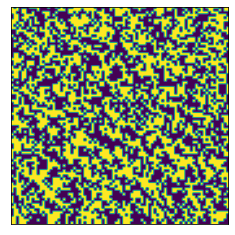
\includegraphics[width=0.19\linewidth]{images/noise/PongNoFrameskip-v4_gsm_ppo_eps_0.1.png}}
  \subcaptionbox{\label{fig:subfig-b}}
    {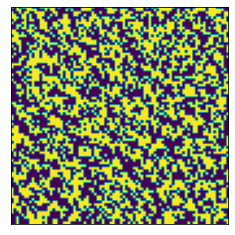
\includegraphics[width=0.19\linewidth]{images/noise/PongNoFrameskip-v4_gsm_ppo_eps_0.01.png}}
    \subcaptionbox{\label{fig:subfig-c}}
    {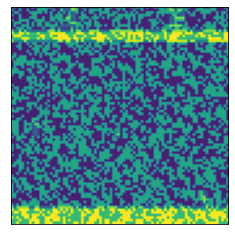
\includegraphics[width=0.19\linewidth]{images/noise/PongNoFrameskip-v4_gsm_ppo_eps_0.001.png}}
    \subcaptionbox{\label{fig:subfig-d}}
    {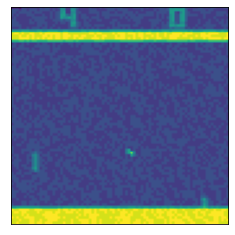
\includegraphics[width=0.19\linewidth]{images/noise/PongNoFrameskip-v4_gsm_ppo_eps_0.0001.png}}
    \subcaptionbox{\label{fig:subfig-e}}
    {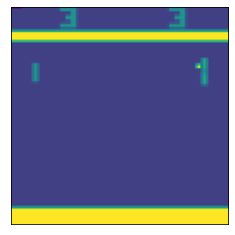
\includegraphics[width=0.19\linewidth]{images/noise/PongNoFrameskip-v4_gsm_ppo_eps_0.1_ori.png}}
    \subcaptionbox{\label{fig:subfig-f}}
    {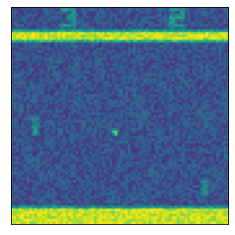
\includegraphics[width=0.19\linewidth]{images/noise/PongNoFrameskip-v4_pgda_ppo_eps_0.1.png}}
    \subcaptionbox{\label{fig:subfig-g}}
    {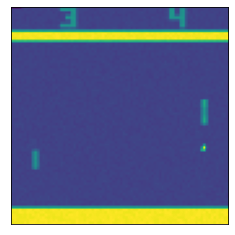
\includegraphics[width=0.19\linewidth]{images/noise/PongNoFrameskip-v4_pgda_ppo_eps_0.01.png}}
    \subcaptionbox{\label{fig:subfig-h}}
    {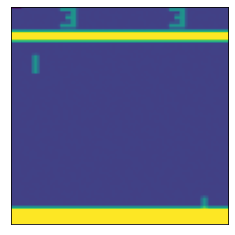
\includegraphics[width=0.19\linewidth]{images/noise/PongNoFrameskip-v4_pgda_ppo_eps_0.001.png}}
    \subcaptionbox{\label{fig:subfig-i}}
    {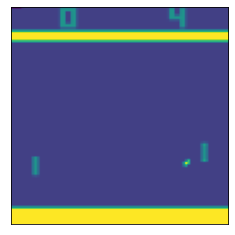
\includegraphics[width=0.19\linewidth]{images/noise/PongNoFrameskip-v4_pgda_ppo_eps_0.0001.png}}
    \subcaptionbox{\label{fig:subfig-j}}
    {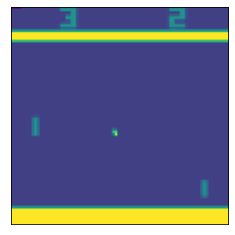
\includegraphics[width=0.19\linewidth]{images/noise/PongNoFrameskip-v4_pgda_ppo_eps_0.1_ori.png}}
  \caption{{\bf First row}: Comparison of the effect of noise injections on Pong environment observations with different strength of perturbations. The most right one is a clear observation and from the right to the left have been injected noise with increasing perturbations \(\epsilon=[0.1, 0.01, 0.001, 0.0001]\). Perturbations have been crafted with FGSM attacking a policy trained with PPO. {\bf Second row}: Comparison of the effect of noise injections on Pong environment observations with different strength of perturbations. The most right one is a clear observation and from the right to the left have been injected noise with increasing perturbations \(\epsilon=[0.1, 0.01, 0.001, 0.0001]\). Perturbations have been crafted with PGD attacking a policy trained with PPO.}
  \label{figure:pong-noise}
\end{figure}

\section{Number of attacked policies}
One of the major difficulties encountered while carrying out this thesis work is the computation time taken to run all the experiments. For the first experiment have been evaluated 5 policy attacks against 3 reinforcement learning algorithms trained on 2 environments. Each policy has been attacked 4 times corresponding to the four curves shown on each chart: attacking without transferability, attacking a surrogate policy, and attacking two different surrogate algorithms. Each curve has been drawn out of 10 different attack frequencies corresponding to ten points along the \(x\)-axis. Uniform attack, since it is the fastest attack, has its corresponding curves containing 20 points. Moreover, each point has been computed as average of 10 runs. Thus, in total have been attacked at least \(5*3*2*4*10*10=12000\) policies. The second experiment instead evaluates 2 policy attacks against 3 reinforcement learning algorithms trained in a single environment. Similarly, each policy has been attacked 4 times corresponding to the four curves shown on each chart as in the previous experiment. Given that each curve is composed of 10 points averaged over 10 runs, in total have been attacked at least \( 2*3*1*4*10*10=2400\) policies. Finally in the third experiment have been evaluated 6 policies trained with DQN where 5 of them were defended with a defense mechanism and trained on the Pong environment. Each policy has been attacked with 3 different white-box attack methods and each curve is composed of 20 points taken over an average of 10 runs. The experiment has been conducted on both targeted and untargeted threat models. Hence, in total have been attacked \(6*3*2*20*10=7200\) policies. Hence, the whole work includes a total of 12000+2400+7200=21600 policy attacks. It took about two months using between 4 and 8 GeForce GTX TITAN X GPUs. In practice, more experiments have been conducted while tuning the attacks' hyper-parameters and verifying the correctness of all the implemented attacks.

\section{Implementation details}
In this section, we are going to discuss the details relative to the implementation of the evaluated reinforcement learning algorithms, the policy attacks, and the image attacks. The Github repository containing the code to obtain the results presented in this thesis is available at the following address: \url{https://github.com/davide97l/rl-policies-attacks-defenses}. It has been developed with Pytorch but relies on other frameworks, each specialized in a different task. The reinforcement learning algorithms have been taken from the framework \href{https://github.com/davide97l/rl-policies-attacks-defenses}{Tianshou} \cite{tianshou} developed by \href{http://ml.cs.tsinghua.edu.cn/}{TSAIL}. It consists of a reinforcement learning platform based on pure PyTorch and with support to parallelized environments. Image adversarial attacks have been taken from \href{https://github.com/BorealisAI/advertorch}{Advertorch} \cite{ding2019advertorch} developed by \href{https://www.borealisai.com/en/}{BorealisAI}. Advertorch is a Python toolbox for adversarial robustness research also based on PyTorch. Given that the model interface required by Advertorch is different from the one required by the model trained with Tianshou, it has been created an adapter class to adapt Tianshou models to Advertorch models. The two simple image defenses, namely JPEG conversion and feature squeezing have been implemented from scratch. Policy adversarial training has been developed from scratch and integrated into Tianshou. It expands the Tianshou classes implementing the training procedure of the normal policies to defend them with adversarial training. Policy attacks have also been implemented from scratch and made compatible with Tianshou. Their modularized code allows to easily develop new attacks by expanding a base class or any of the existing policies. Hence, the result of this work is also a framework to test the robustness of reinforcement learning trained policies. Finally, the Atari environments have been taken from the Gym library developed by \href{https://openai.com/}{OpenAI}. The same library also includes other well-studied environments made publicly available to the AI community.